\documentclass[prl,aps,superscriptaddress,twocolumn]{revtex4-1}
\usepackage{graphicx}
\usepackage{amsfonts}
\usepackage{amssymb}
\usepackage{bm}
\usepackage{bbold}
\usepackage{color}
\usepackage[breaklinks]{hyperref}
\usepackage{epstopdf, epsfig}

% Mathematical definitions
\newcommand{\bX}{\bm X}
\newcommand{\bu}{\bm u}
\newcommand{\bF}{\bm f}

% Addresses
\newcommand{\cemef}{Ecole Nationale Sup\'erieure des Mines de Paris, PSL University, CNRS, Cemef, Sophia-Antipolis, France}
\newcommand{\inria}{Universit\'e C\^ote d'Azur, Inria, CNRS, Cemef, Sophia-Antipolis, France}

\begin{document}
\title{Steering undulatory microswimmers in a moving fluid through machine learning}
\author{Rapha\"{e}l Chesneaux} \affiliation{\cemef}
\author{La\"etitia Giraldi} \affiliation{\inria} 
\author{J\'er\'emie Bec} \affiliation{\cemef} \affiliation{\inria}
\begin{abstract}
r\'esum\'e
\end{abstract}

\maketitle

%%%%%%%% INTRODUCTION %%%%%%%%%%%%
\section{Introduction}
Applications of microswimmers. Microorganisms such as bacteria or plankton are natural examples of self-propelled particles. They often inspire the design of artificial devices used for industrial micro-manufacturing, toxic waste disposal, targeted drug delivery or localized diagnostics~\cite{wu2020medical}. Many questions remain open on how these micro-swimmers optimize their movement, and in particular how they behave in complex flows comprising walls or having non-Newtonian properties.

Swimming vs. Navigation. In the first case, mainly fluid-structure interactions in creeping flows described by the Stokes equation~\cite{berti2020swimming}, optimal control, biomimetics~\cite{borazjani2009numerical,cohen2010swimming}, problem of swimming in a complex fluid~\cite{shen2011undulatory}. Importance of hydrodynamics stressed in~\cite{daddi2021hydrodynamics}, in particular in the presence of obstacles. Complicated carrier flows has been mostly considered for navigation problems where the swimming mechanisms are oversimplified but one rather focuses on how to adjust macroscopic active features of the swimmers in order to optimize its long-term displacement. In this case, use of machine learning has proved efficiency~\cite{cichos2020machine}, effect of obstacles, of a potential barrier~\cite{schneider2019optimal}, of the fluid flow chaoticity~\cite{colabrese2017flow,alageshan2020machine}. Here we want to address the two problems at once. 

%%%%%%%% MODEL %%%%%%%%%%%%
\section{Model for undulatory locomotion}
We consider that the swimmers are elongated, flexible and inextensible. They are moreover very thin, meaning that their cross-section diameter $d$ is much smaller than their length $\ell$. This assumption allows describing their interactions with the fluid in terms of the slender-body theory~\cite{lindner2015elastic}. The swimmer is moreover embedded in an incompressible fluid flow whose unperturbed velocity field is denoted by $\bu(\boldsymbol{x},t)$. The swimmer's conformation at time $t$ is characterized by a curve $\bX(s,t)$ parametrized by its arc-length $s\in[-\ell/2,\ell/2]$. In the limit of very small inertia, its dynamics is given by the over-damped limit obtained by balancing the viscous drag to the other forces in the slender-body equation, so that
\begin{equation}
  \zeta\,\mathbb{R}\left[\partial_t \bX-\bu(\bX,t)\right] = \partial_s(T\partial_s \bX) - K\,\partial_s^4 \bX + \bF(s,t).
  \label{eq:vel_fib}
\end{equation}
The viscous force involves the drag coefficient $\zeta = 8\pi\nu\rho_{\rm f}/[2\log(\ell/d)-1]$ (with $\nu$ the fluid kinematic viscosity and $\rho_{\rm p}$ its density) and the local Oseen's resistance tensor $\mathbb{R} = \mathbb{1} -(1/2)\,\partial_s\bX\,\partial_s\bX^{\mathsf{T}}$. The first force in the right-hand side is the tension whose amplitude $T$ is determined by the inextensibility constraint $|\partial_s\bm X(s,t)| = 1$, valid at all time along the swimmer. The second term is the bending elasticity force which depends upon the swimmer's flexural rigidity $K$ (product of Young's modulus and inertia). The last term denoted $\bF$ is an internal force that is prescribed to account for the so-called active behaviours of the swimmer and in particular its locomotion. Comment here on the various physical quantities and non-dimensional parameters.

Specify the locomotion force: We choose it of the form $\bF = A\,\cos(\nu\,s-\omega\,t)\,\bm p$ with $\bm p$ a unit vector chosen orthogonal to the direction  in which the swimmer needs to move. We write the forcing amplitude as $A = \alpha\,\zeta\,\omega/\nu$ where $\alpha$ is a dimensionless parameter that controls its strength. Considerations on the global conservation of momentum, that imply in particular $\nu = 2\,\pi\,k/\ell$ with $k$ integer.

State the problem: We want the swimmer to swim as fast as possible toward $x>0$. This amounts to choose $\bm p$ perpendicular to $\bm e_x$. Talk about the symmetry $x\mapsto-x$.

\begin{figure}[ht]
  \centerline{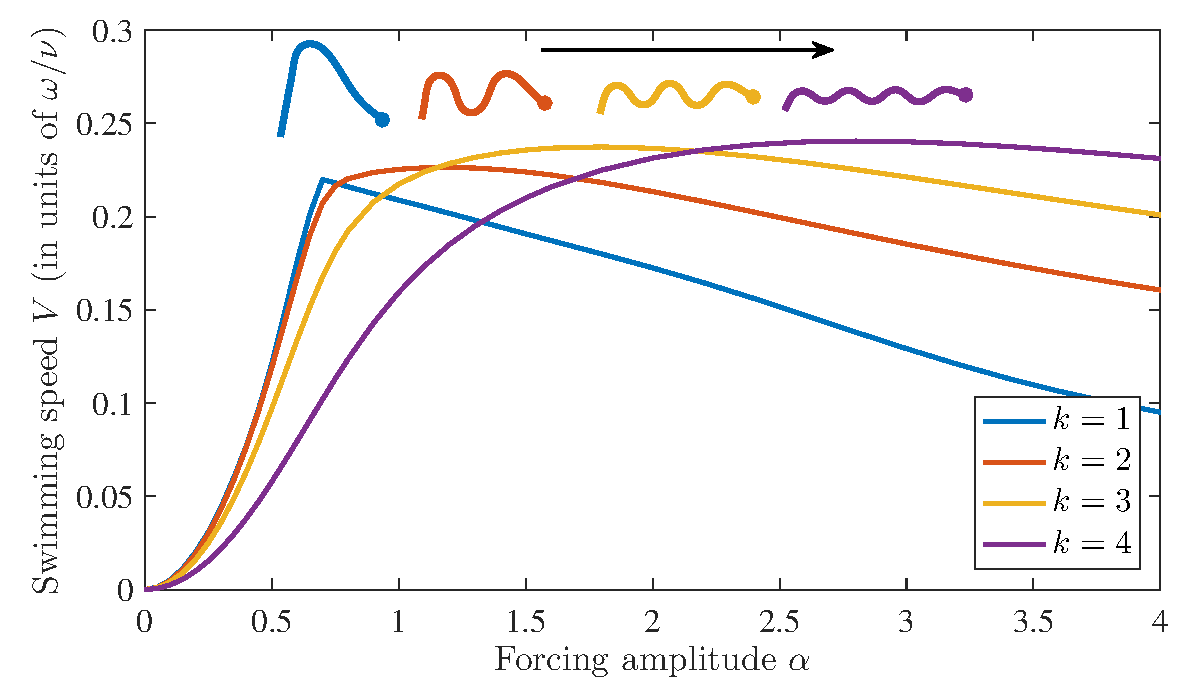
\includegraphics[width=\columnwidth]{swimming_speed_nofluid}}
  \caption{\label{fig:swimming_speed_nofluid} Swimming speed as a function of the forcing amplitude parameter $\alpha$ for different wavenumbers such as $\nu = 2\,\pi\,k/\ell$ and a fixed phase velocity $\omega/\nu$.}
\end{figure}
Explain that we find that the swimmer moves with a velocity proportional to the phase velocity of the undulation $\omega/\nu$, with some qualitative explanation why, but no analytic results on the dependence of the swimming speed on the parameters. That's why we rely on numerics, with the results shown in Fig.~\ref{fig:swimming_speed_nofluid}.
Some words on the numerical method (second-order finite differences, second-order time marching, penalization for inextensibility), citing~\cite{tornberg2004simulating}. Specify the numerical parameters: discretization of the fiber over $N_s = 201$ points, time-step $\delta t$ (chosen in our simulations to $\delta t = 5\times10^{-4}$).

%%%%%%%% Introducing the flow %%%%%%%%%%%%
\section{Cellular flow}

From now on we focus on two dimensions. Introduce the cellular flow $\bm u = (-\partial_y\Psi,\partial_x\Psi)$ with the periodic stream function $\Psi(x,t) = (L\,U/\pi)\,\cos(\pi\,x/L)\,\cos(\pi\,y/L)$. Cells of size $L$, mimicking eddies. The velocity amplitude $U$ is to be compared to the swim velocity. Even if the motion of tracers in such a flow is non-chaotic, the swimmer's dynamics is.  

Naive strategy: either undulate in the $y$ direction if the swimmer is facing $x>0$, do otherwise nothing. Problem with trapping in vortex cores.

%%%%%%%% Learning %%%%%%%%%%%%
\section{\textit{Q}-learning}

We use the classical $Q$-learning algorithm with a set of discrete states $\mathcal{S}$ and discrete actions $\mathcal{A}$. The policy is described by the $Q$-table, which assigns at time $t$ to each couple $(s,a)\in \mathcal{S}\times \mathcal{A}$ a mark $Q_t(s,a)$. The action $a_t$ taken at time $t$ is such that it maximizes $Q_t(s_t,\cdot)$.

Specify the states and the action and express the naive strategy in terms of a $Q$-table.

The learning algorithm is based on the classical value-iteration update of the Bellman equation, namely
\begin{eqnarray}
    Q_{t+\Delta t}(s_t,a_t) &=& (1-\alpha\,\Delta t)\,Q_{t}(s_t,a_t) \nonumber\\
    &&+ \alpha\,\Delta t\,\left[r_t + \gamma\,\max_a Q_{t}(s_{t+\Delta t},a) \right],
    \label{eq:Qlearning}
\end{eqnarray}
where $\alpha$ denotes the learning rate, $\gamma$ the discount factor, and $r_t$ is the reward, which in our case is defined as the distance travelled in the $x$ direction by the swimmer's center of mass, namely $r_t = \bar{x}(t+\Delta t)-\bar{x}(t)$ with $\bar{x}(t) = (1/\ell) \int \bm e_x\cdot\bm X(s,t)\,\mathrm{d}s$.
\begin{figure}[ht]
  \centerline{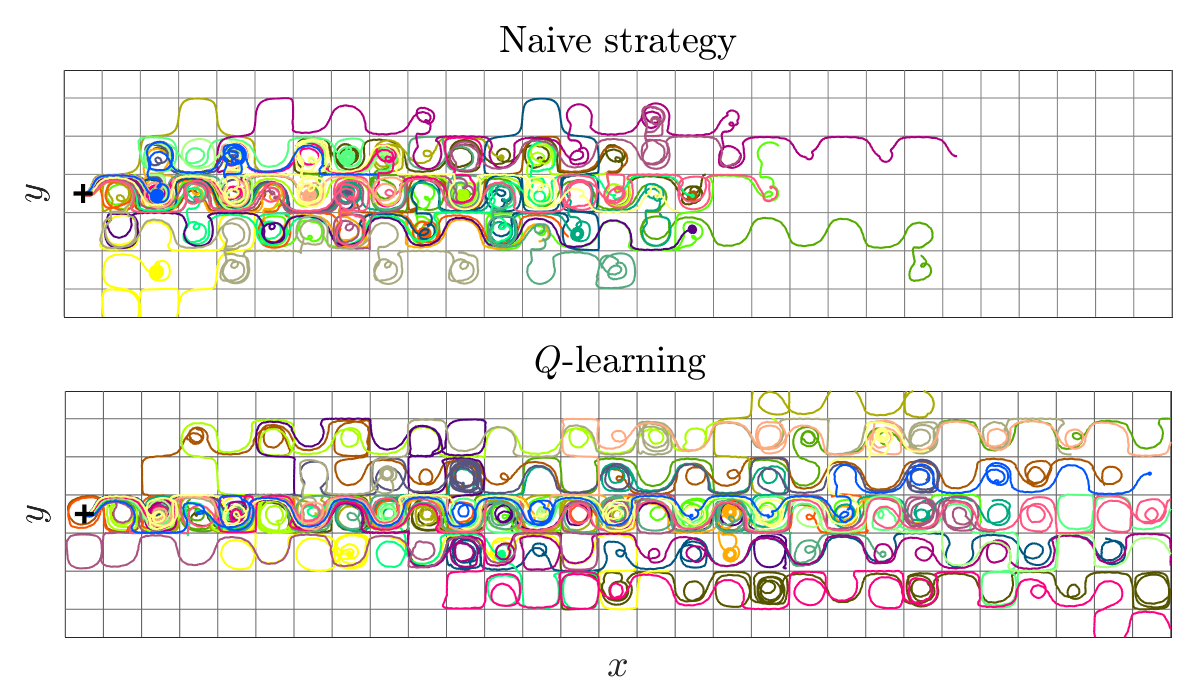
\includegraphics[width=\columnwidth]{compare_traj}}
  \caption{\label{fig:compare_traj} Horizontal displacement for different realizations of  learning, together with the average shown as a bold solid line, and the interval defined by the standard error shown as dashed lines.}
\end{figure}

\begin{figure}[ht]
  \centerline{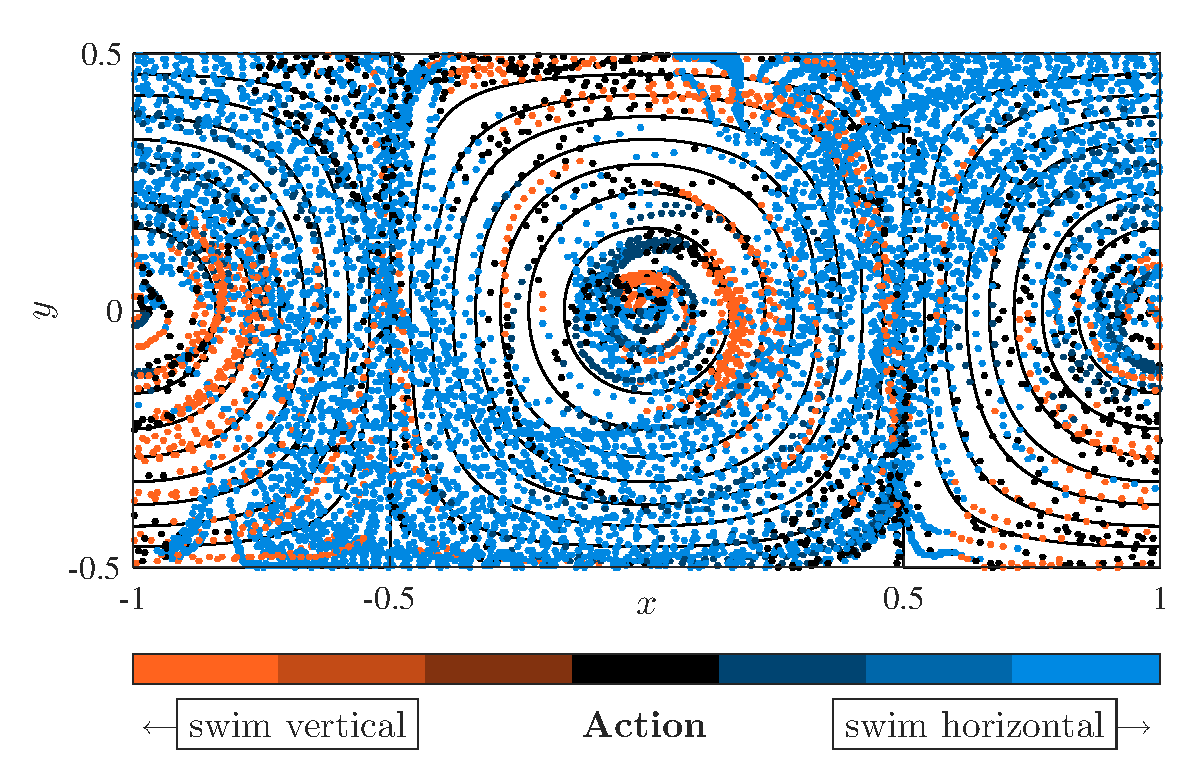
\includegraphics[width=\columnwidth]{traj_centerofmass}}
  \caption{\label{fig:traj_centerofmass} Typical trajectory of the swimmer's center of mass obtained after learning. The positions have been here folded to account for periodicity. The colors correspond to the different actions taken by the swimmer, ranging from red (swimming with $\alpha = 1$ in the $y$ direction) to blue (swimming with $\alpha = 1$ in the $x$ direction).}
\end{figure}

\begin{figure}[ht]
  \centerline{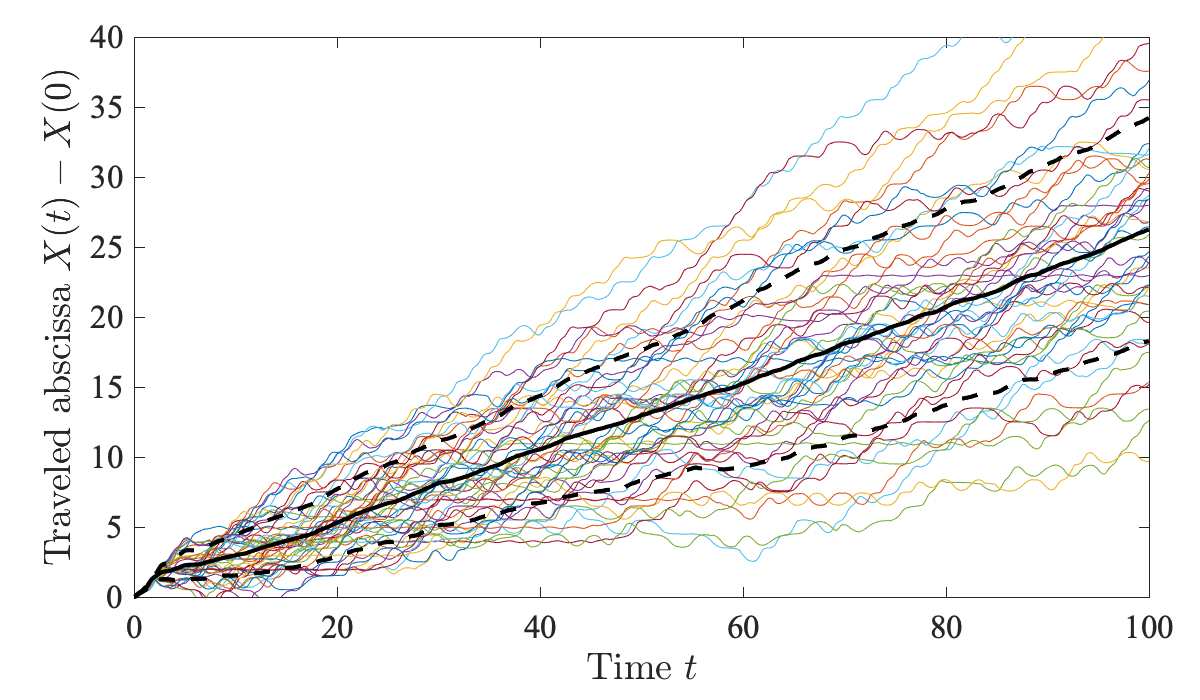
\includegraphics[width=\columnwidth]{travel_learn_diffreal}}
  \caption{\label{fig:travel_learn_diffreal} Horizontal displacement for different realizations of  learning, together with the average shown as a bold solid line, and the interval defined by the standard error shown as dashed lines.}
\end{figure}


\bibliography{biblio}

\end{document}
